\chapter{專題設計}
\renewcommand{\baselinestretch}{10.0} %設定行距
\pagenumbering{arabic} %設定頁號阿拉伯數字
\setcounter{page}{2}  %設定頁數
\fontsize{14pt}{2.5pt}\sectionef

\section{尺寸規定}
在 https://mde.tw/cd2023/content/pj3.html 中規定球場及球員的大小及重量。\\
1. 足球規格:球為白色、直徑 0.1m、重量 0.5kg\\
2. 足球場地:長 4m x 寬 2.5m\\
3. 球門規格:長 0.6m, 高 0.3m, 寬 0.1m\\
4. 球員尺寸範圍:長寬高各 0.2m, 重量 5kg。\\

\section{建立球員}
本組使用 CoppeliaSim 內的 primitive shape 來製作車子,之所以使用簡單的形狀來製作車子是因為在模擬時車子細節太複雜會導致模擬運行速度變慢。由於初始的機器人為球型會導致在碰撞時容易翻倒,所以經過本組討論後在後續車體改良中更改為長方體使球員不容易翻倒。\\
\begin{figure}[hbt!]
\begin{center}
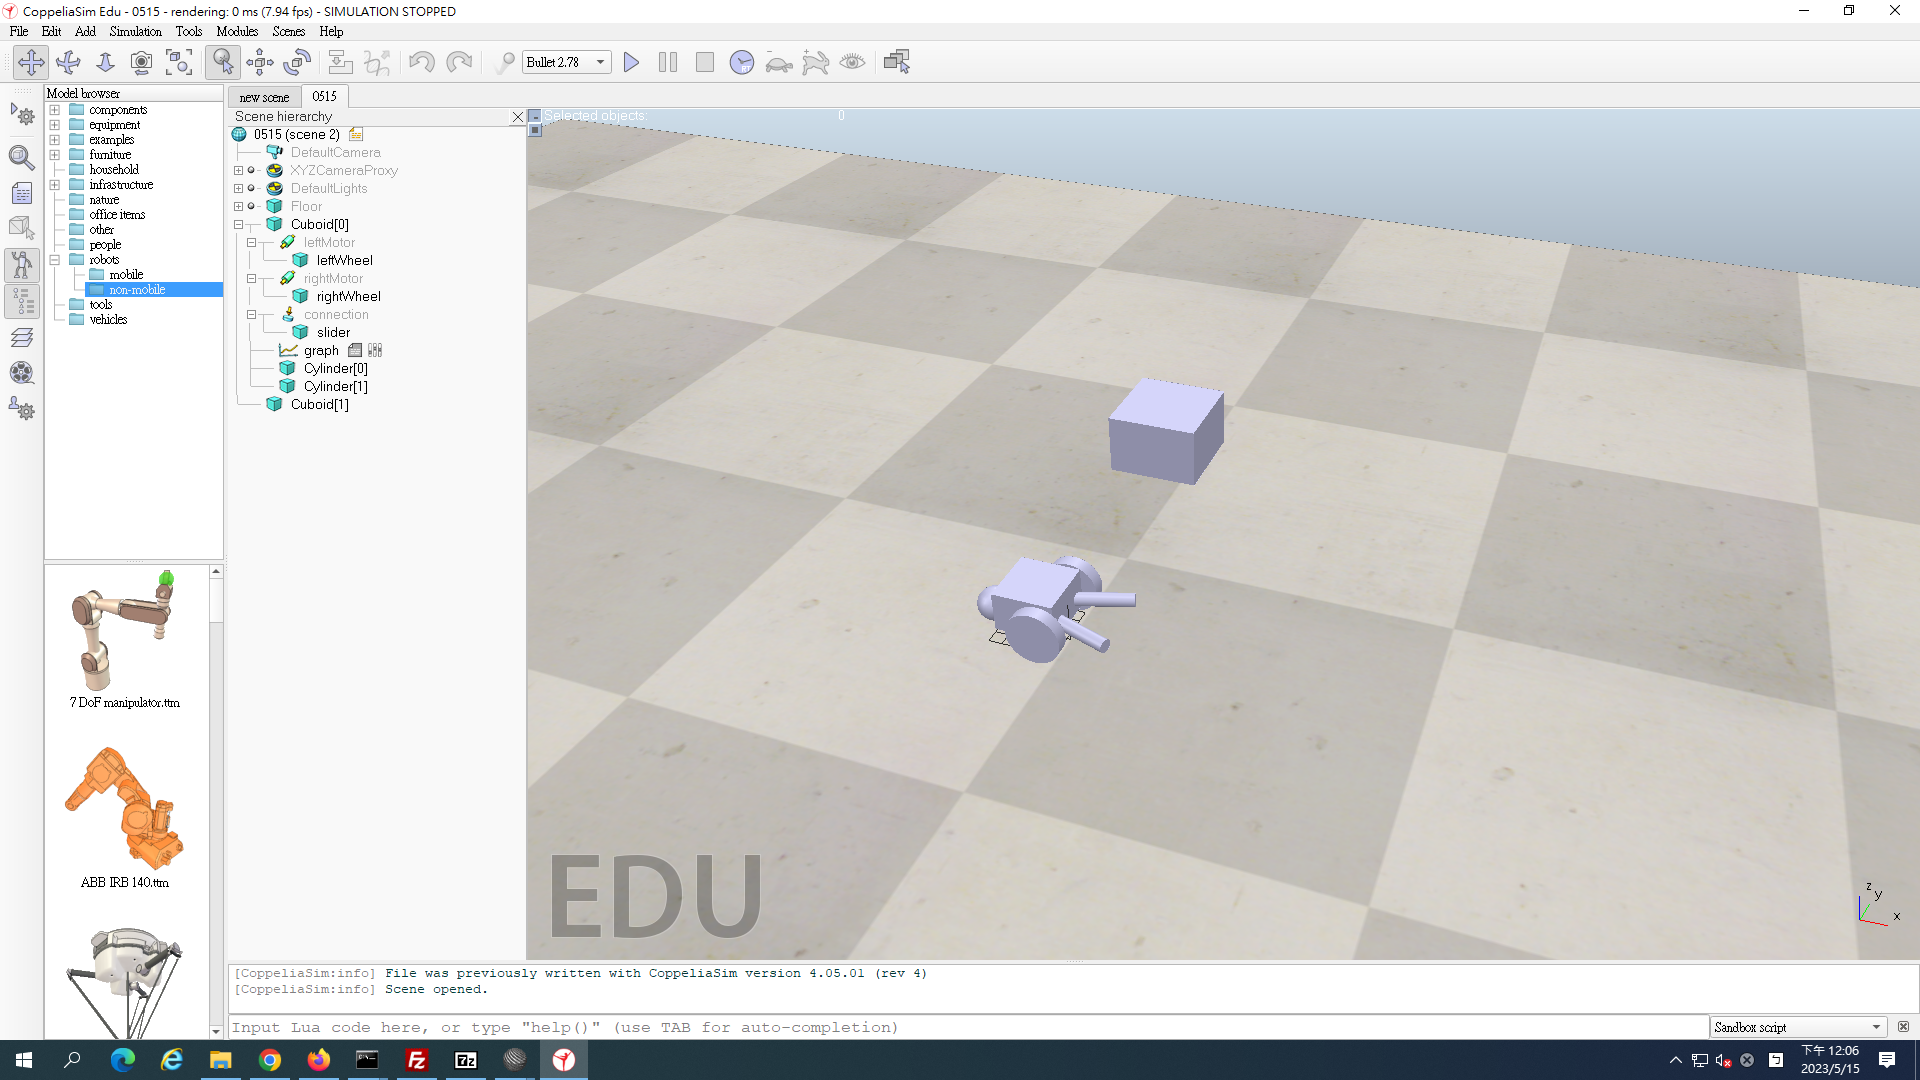
\includegraphics[width=10cm]{0515}
\caption{\Large 第一版車體}\label{車體}
\end{center}
\end{figure}

在執行控制車子程式時在移動左右轉彎時馬達產生偏移,後來發現是馬達座標設定錯誤直接而修改了定位,並且加上顏色及背號。\\
\begin{figure}[hbt!]
\begin{center}
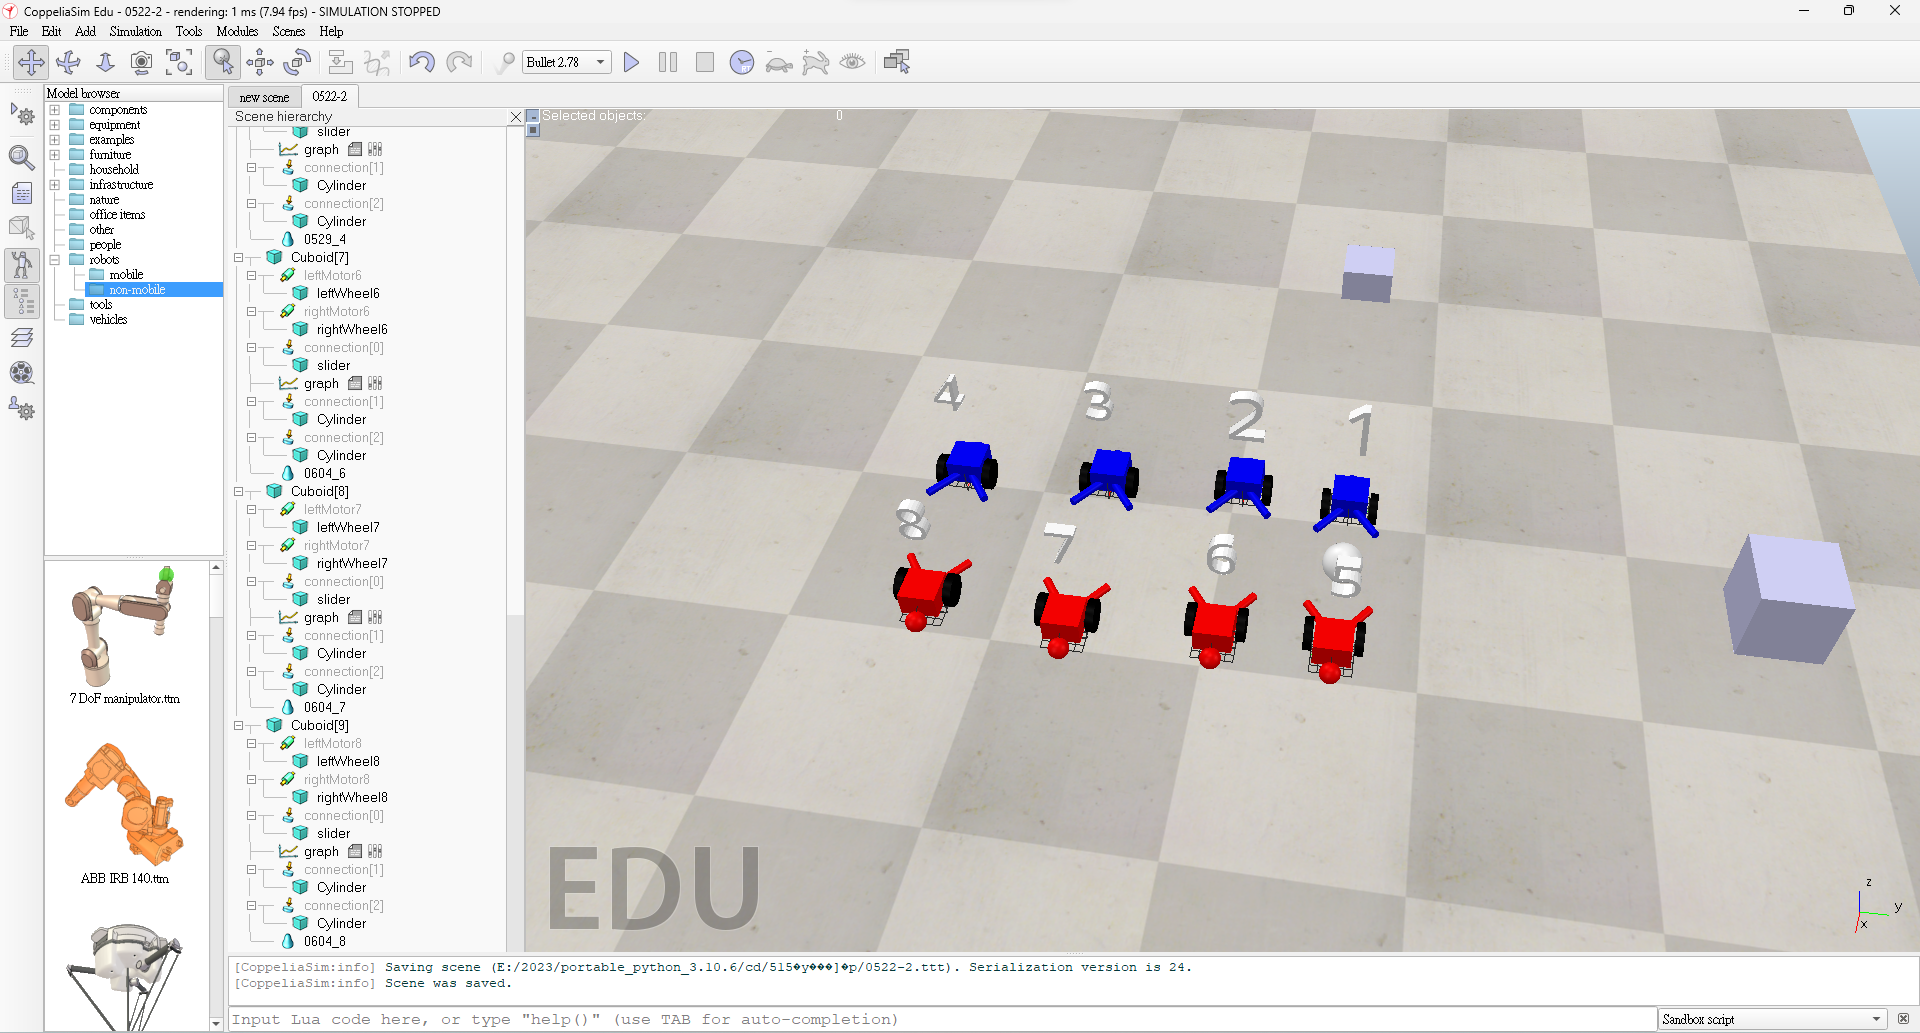
\includegraphics[width=12cm]{0604-1}
\caption{\Large 車體導入場景}\label{車體導入場景}
\end{center}
\end{figure}

\section{建立記分板}
本課程規定除了採用 LED 顯示計分外, 也要建立機械轉盤傳動計分系統。\\
LED 顯示計分是採用 NX 繪製出 stl 檔再導入 CoppeliaSim 中而程式部分後續會說明。\\
\begin{figure}[hbt!]
\begin{center}
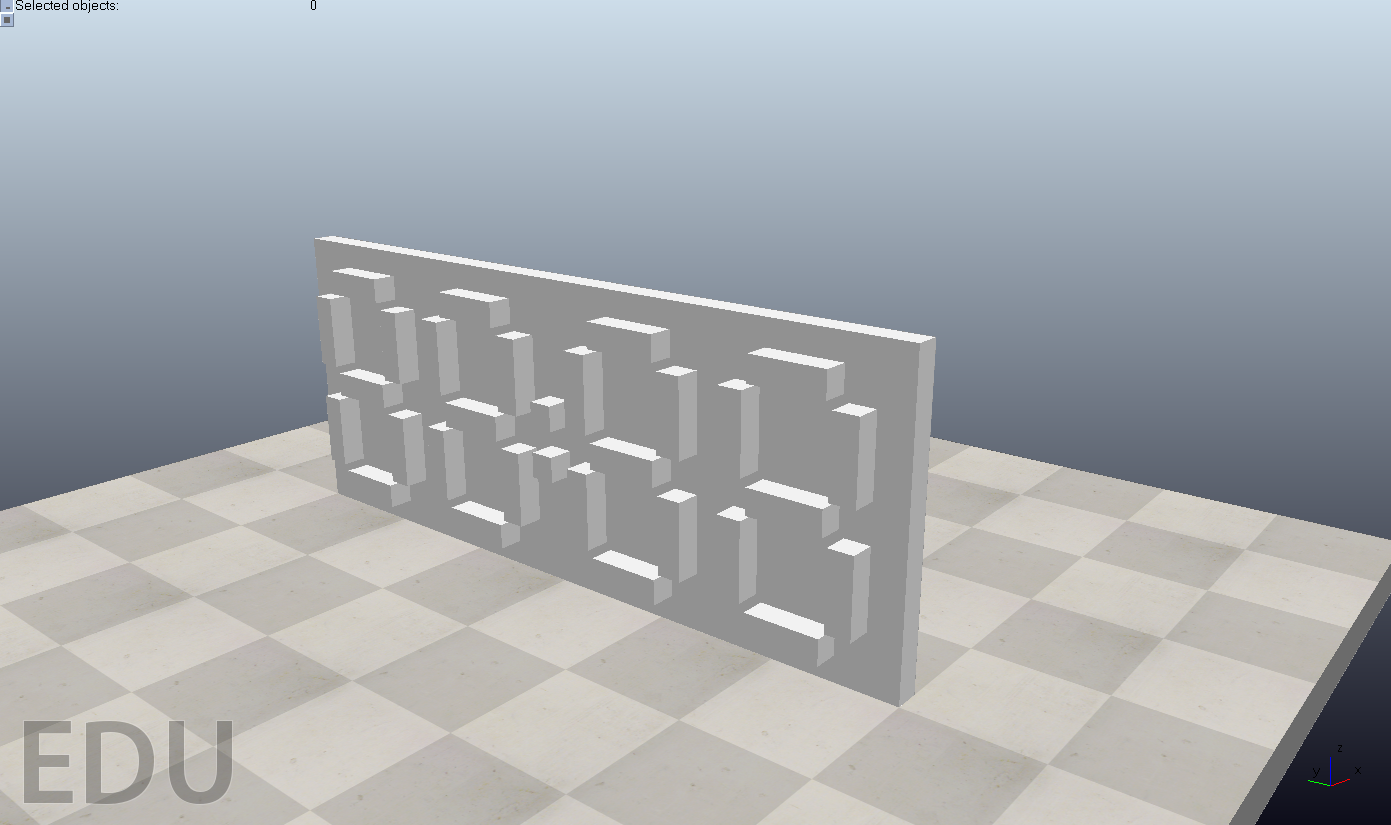
\includegraphics[width=10cm]{ledscore}
\caption{\Large 記分板建立}\label{記分板建立}
\end{center}
\end{figure}

機械轉盤傳動計分版是利用 onshape 繪製而成,並更改了顏色,但後續程式無法編譯出來而參考 pj3ag4 的機械式記分板。\\
\begin{figure}[hbt!]
\begin{center}
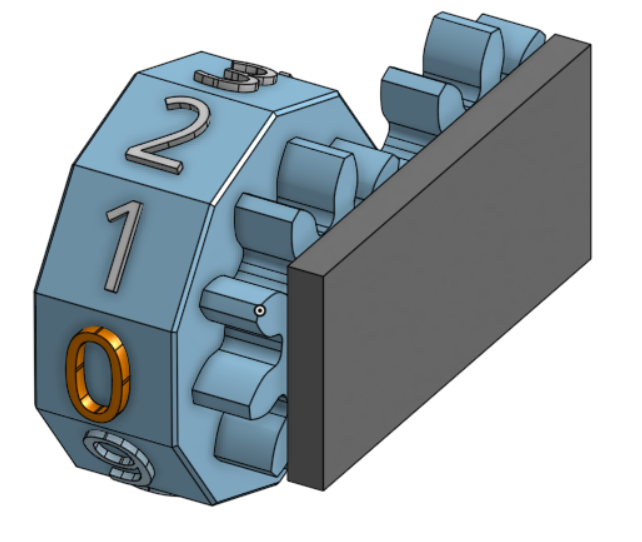
\includegraphics[width=8cm]{輪盤記分板-4-10teeth}
\caption{\Large 初版記分板}\label{初版記分板}
初版記分板 概念是由馬達帶動齒輪10齒輪傳動
\end{center}
\end{figure}
\begin{figure}[hbt!]
\begin{center}
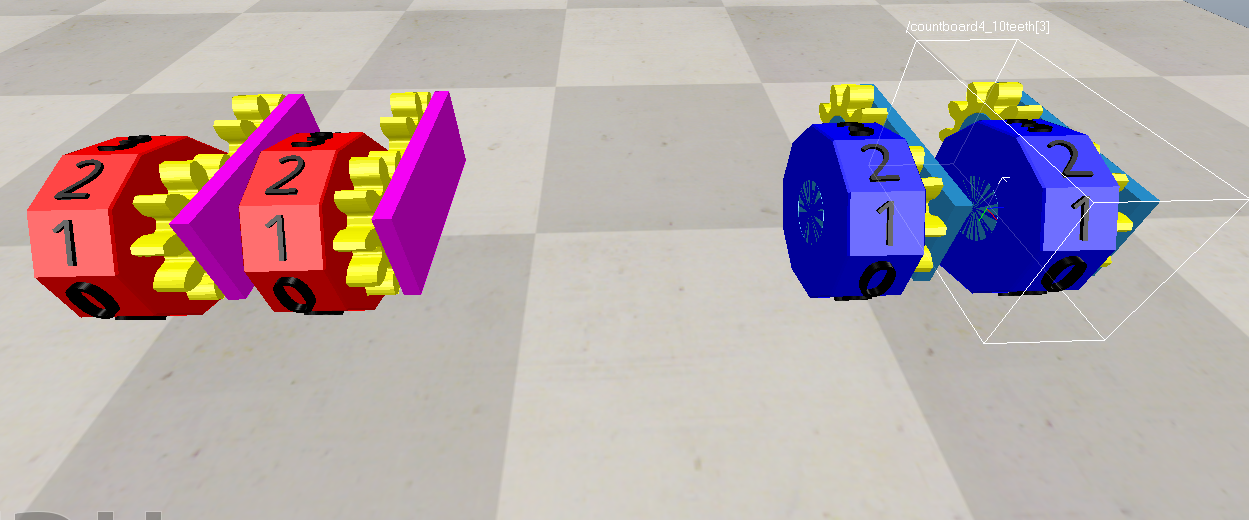
\includegraphics[width=8cm]{Screenshot 2023-05-29 113148.png4-10}
\caption{\Large 匯入記分板}\label{匯入記分板}
\end{center}
\end{figure}
\begin{figure}[hbt!]
\begin{center}
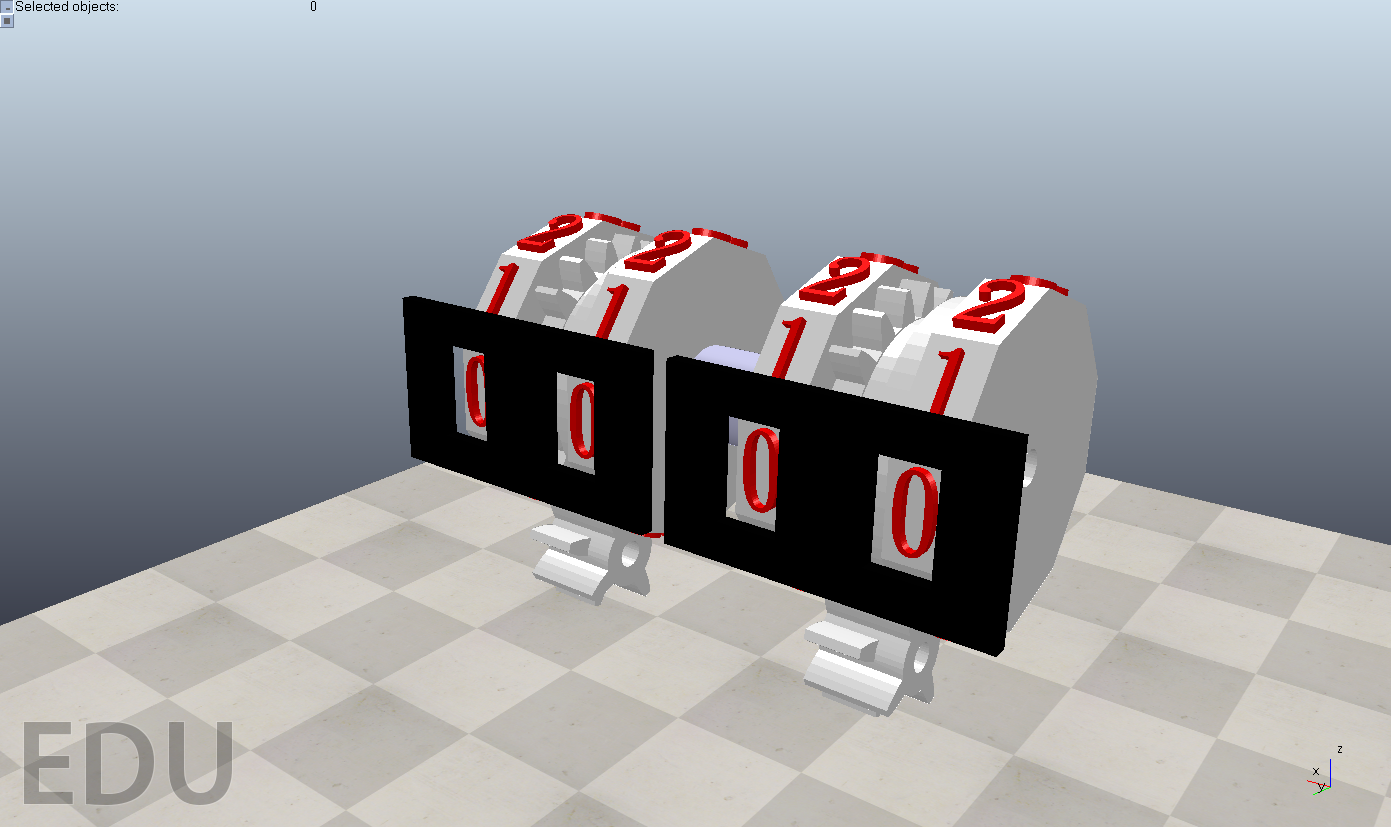
\includegraphics[width=8cm]{scoreboard}
\caption{\Large 匯入第二版記分板}\label{匯入最終版記分板}
最終版記分板 是由齒輪組傳動 20齒及10齒和二階傳動輪組成
\end{center}
\end{figure}
\begin{figure}
\begin{center}
詳細的記分板組成及製作過程 可以參考本組網頁:
\herf{https://mdecd2023.github.io/2a3-pj3ag1/content/輪盤記分板繪製.html}{輪盤記分板繪製}
\end{center}
\end{figure}

\section{建立計時器}
在進行比賽時需要有計時器讓參賽者得知比賽還多久結束,而計時器模型則是沿用記分板之檔案。\\
\begin{figure}[hbt!]
\begin{center}
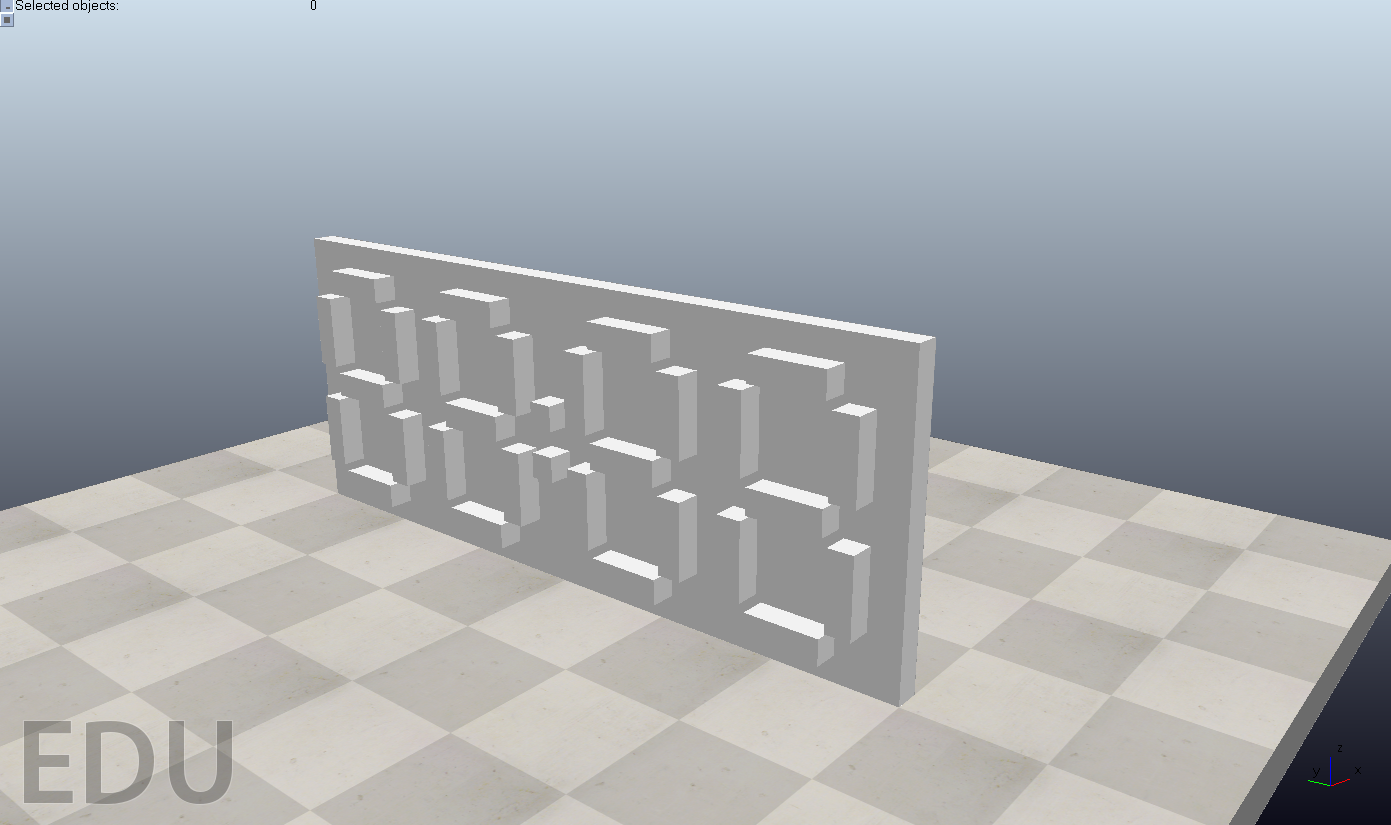
\includegraphics[width=8cm]{ledscore}
\caption{\Large 匯入記時器}\label{匯入記時器}
\end{center}
\end{figure}

\section{建立球場}
我們使用 Onshape 繪製了球場底板及球門,匯入 CoppeliaSim 後更改了顏色。\\
\begin{figure}[hbt!]
\begin{center}
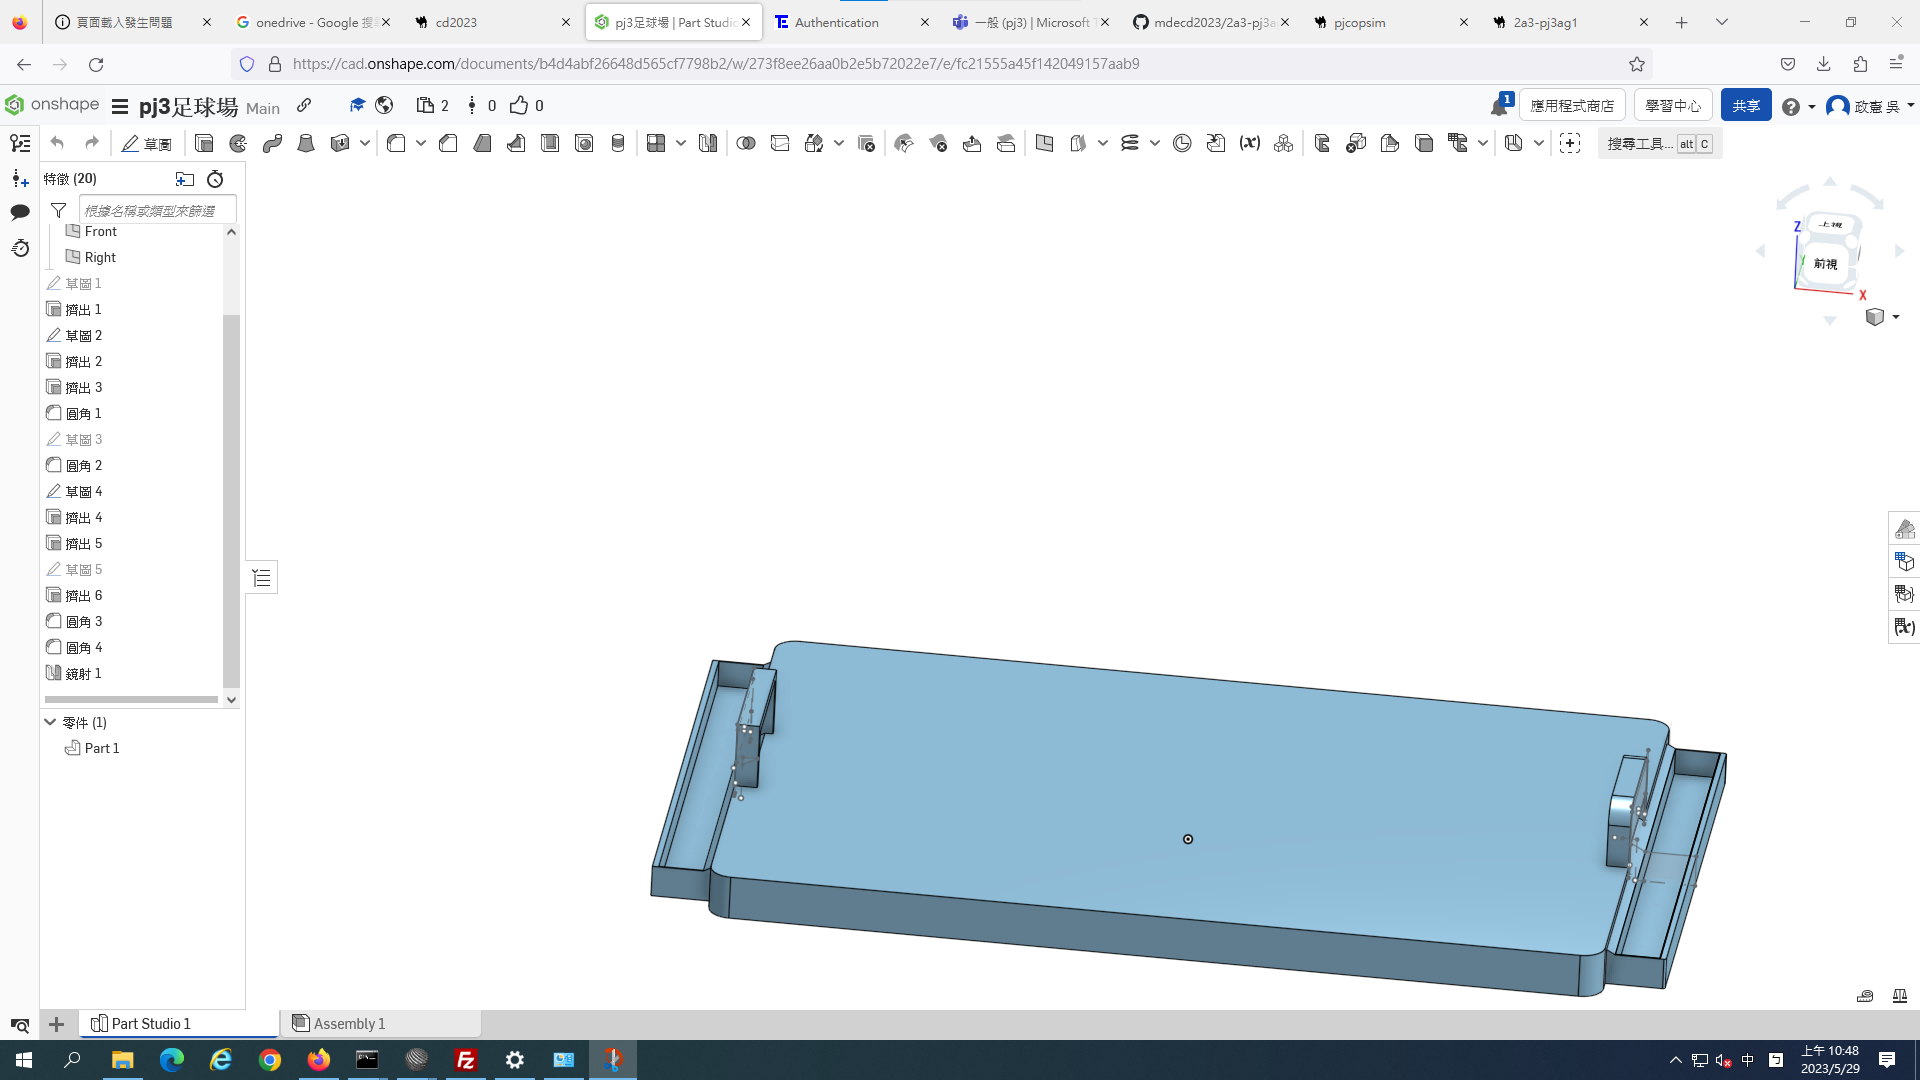
\includegraphics[width=8cm]{33333}
\caption{\Large 球場繪製}\label{球場繪製}
\end{center}
\end{figure}
\begin{figure}[hbt!]
\begin{center}
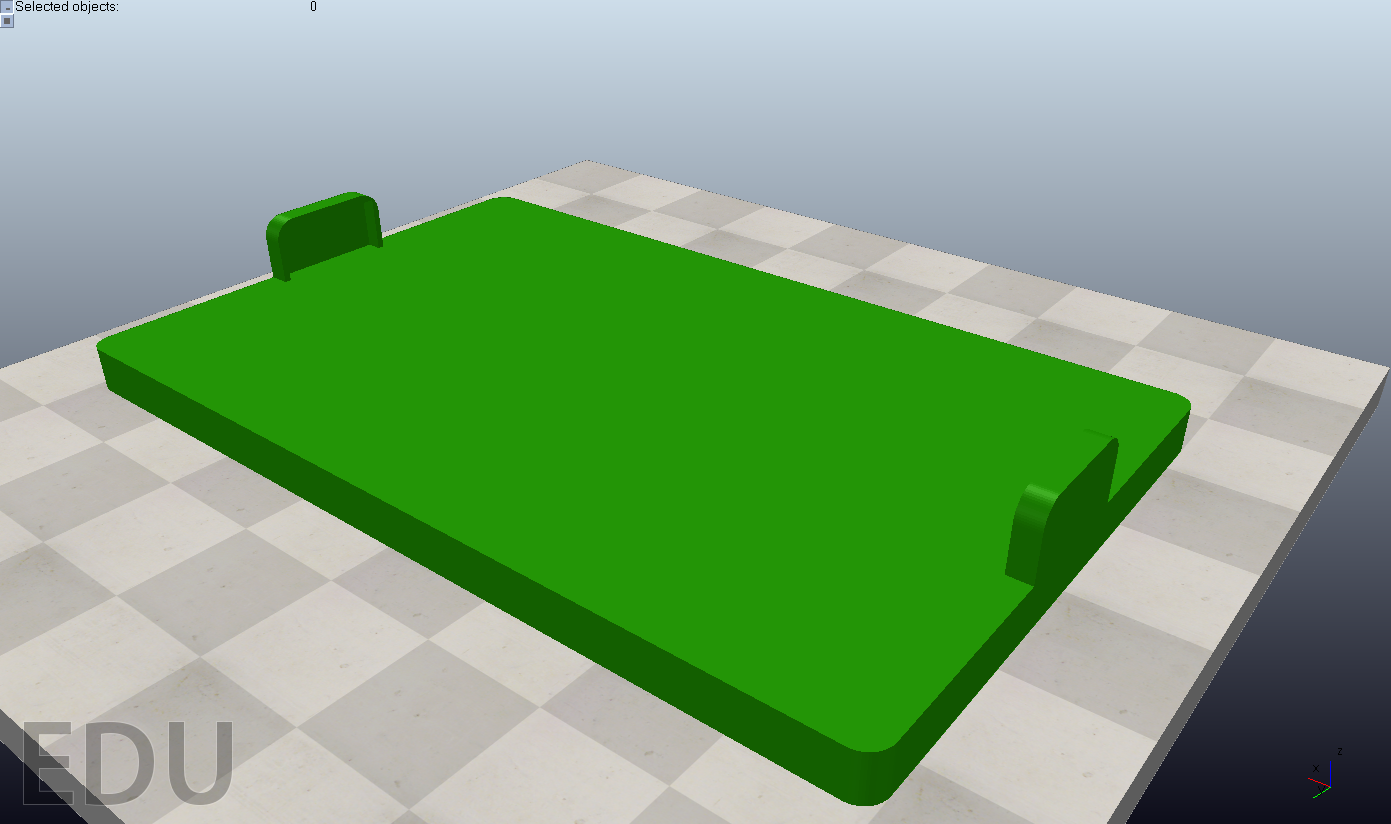
\includegraphics[width=8cm]{board}
\caption{\Large 導入球場}\label{導入球場}
\end{center}
\end{figure}
\newpage

\renewcommand{\baselinestretch}{0.5} %設定行距